\section{Path Selection}
\begin{frame}{Path Selection}
    Path Selection aims to create an ``interesting'' subcomponent \(\tau'\) of \(\tau\). 

    \begin{figure}[H]
        \centering
        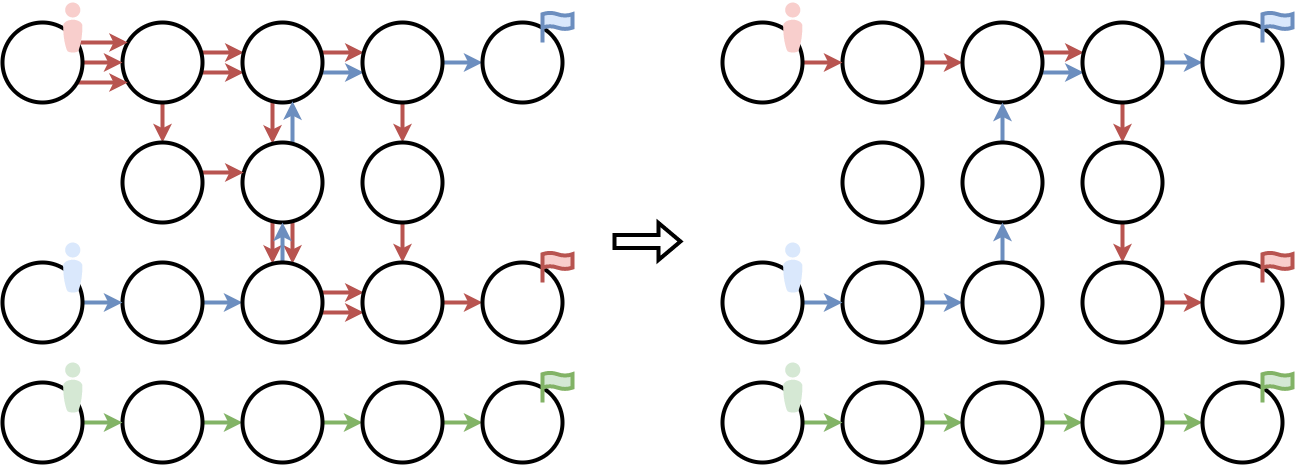
\includegraphics[width=11cm]{img/pm_example_intro.png}
    \end{figure}

\end{frame}


\subsection{Path Elimination}
\begin{frame}{Path Elimination}
    \textbf{  Path Elimination} is the process of the removing paths that exhibit potential issues. 
    
    \begin{block}{Why not find brute force a conflict-free set of paths directly?}
        \(\text{    }\blacktriangleright\) Slow with a lot of agents and paths, we need some preliminary process first
    \end{block}

    Two ways:
    \begin{itemize}
        \item \textbf{Based on heatmaps}
        \item Based on potential conflict
    \end{itemize}

\end{frame}


\subsection{Individual Heatmap}
\begin{frame}[fragile]{Individual Heatmap}
    Individual Heatmap is about projecting likelihood of presence of an agent on vertices
at each step.

    \[
        \phi(\gamma,v,t) = \frac{| \{\pi|\pi \in \gamma,\pi(t) = v\}|}{|\gamma|}
    \]


\end{frame}

\begin{frame}{Individual Heatmap example 1/5}

    \begin{figure}[H]
        \centering
        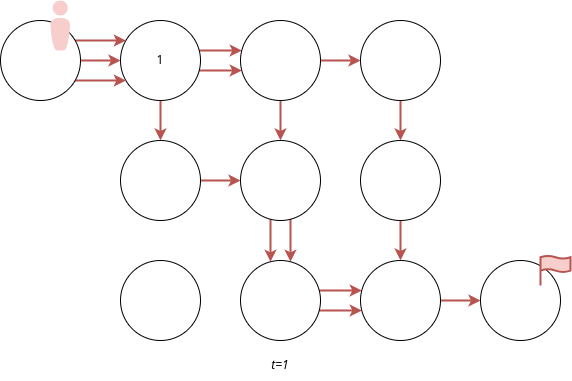
\includegraphics[width=9cm]{img/individual_heatmap_p1.drawio.png}
    \end{figure}
\end{frame}

\begin{frame}{Individual Heatmap example 2/5}
    \begin{figure}[H]
        \centering
        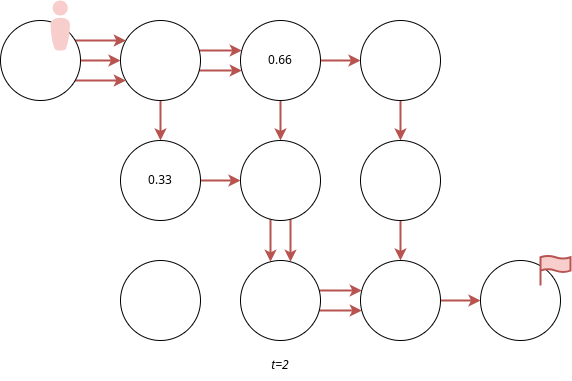
\includegraphics[width=9cm]{img/individual_heatmap_p2.drawio.png}
    \end{figure}
\end{frame}


\begin{frame}{Individual Heatmap example 3/5}
    \begin{figure}[H]
        \centering
        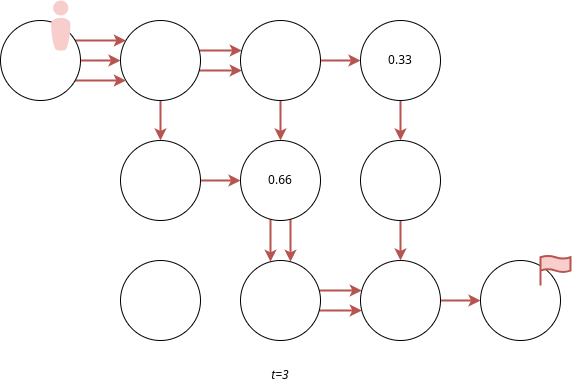
\includegraphics[width=9cm]{img/individual_heatmap_p3.drawio.png}
    \end{figure}
\end{frame}

\begin{frame}{Individual Heatmap example 4/5}
    \begin{figure}[H]
        \centering
        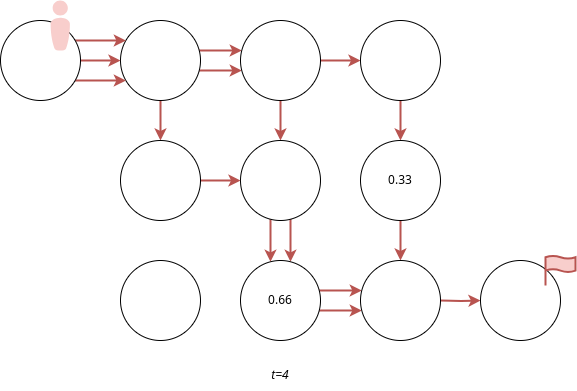
\includegraphics[width=9cm]{img/individual_heatmap_p4.drawio.png}
    \end{figure}
\end{frame}

\begin{frame}{Individual Heatmap example 5/5}
    \begin{figure}[H]
        \centering
        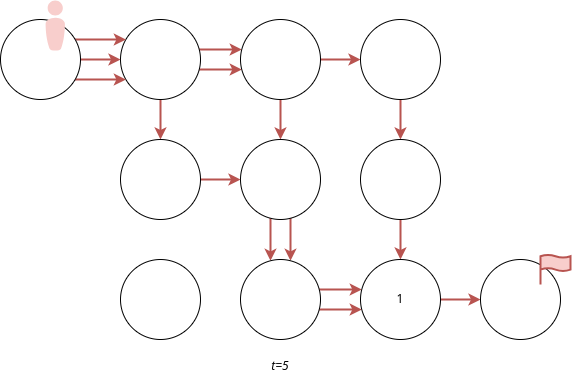
\includegraphics[width=9cm]{img/individual_heatmap_p5.drawio.png}
    \end{figure}
\end{frame}

\subsection{Global Heatmap}

\begin{frame}{Global Geatmap}
    We derive a \textbf{Global Heatmap} (GH) through the aggregation of all Individual Heatmaps
    \[
        \Phi(\tau,v,t) = \frac{ \sum_{\gamma \in \tau}\phi(\gamma,v,t)}{|\tau|}
    \]

    Global Heatmap do not represent a direct indicator of the likelihood of presence but instead an indicator of ``usage of vertices'' by multiple agents
\end{frame}


\begin{frame}{Global Heatmap example 1/5}
    \begin{figure}[H]
        \centering
        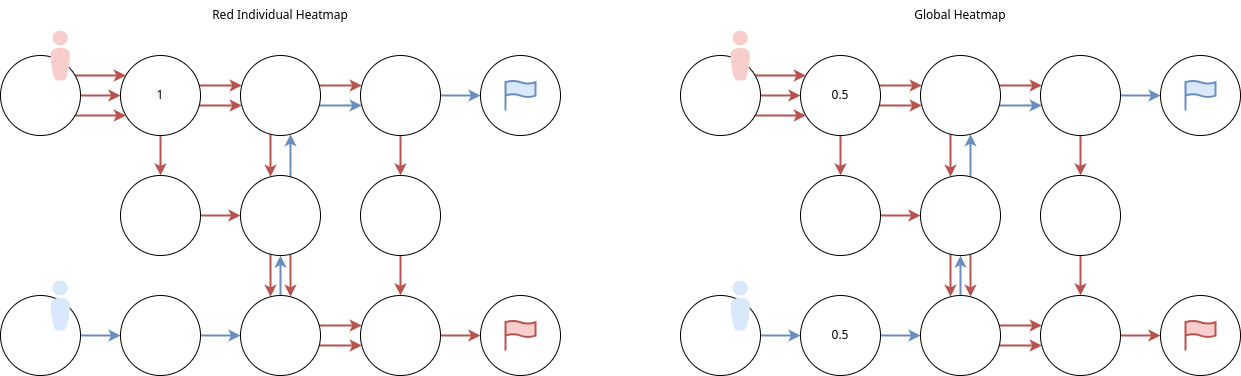
\includegraphics[width=11cm]{img/global_heatmap_p1.drawio.png}
    \end{figure}
\end{frame}


\begin{frame}{Global Heatmap example 2/5}
    \begin{figure}[H]
        \centering
        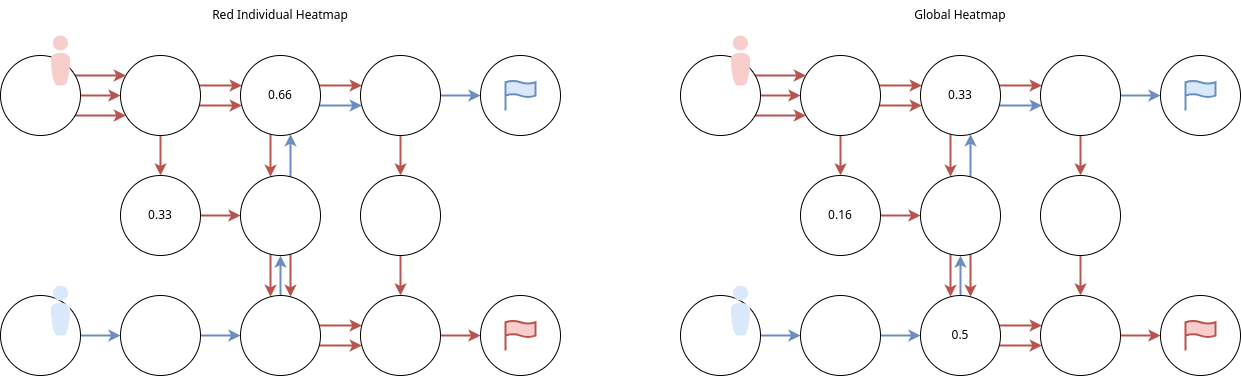
\includegraphics[width=11cm]{img/global_heatmap_p2.drawio.png}
    \end{figure}
\end{frame}



\begin{frame}{Global Heatmap example 3/5}
    \begin{figure}[H]
        \centering
        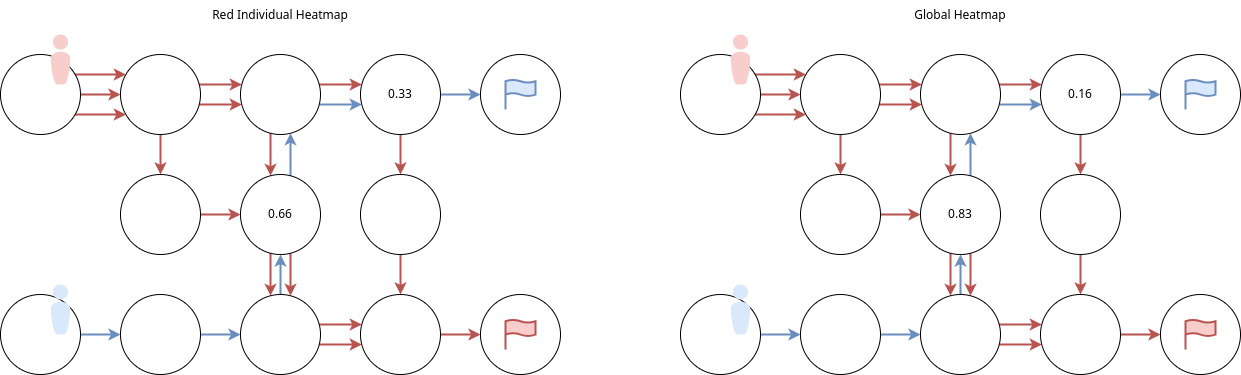
\includegraphics[width=11cm]{img/global_heatmap_p3.drawio.png}
    \end{figure}
\end{frame}


\begin{frame}{Global Heatmap example 4/5}
    \begin{figure}[H]
        \centering
        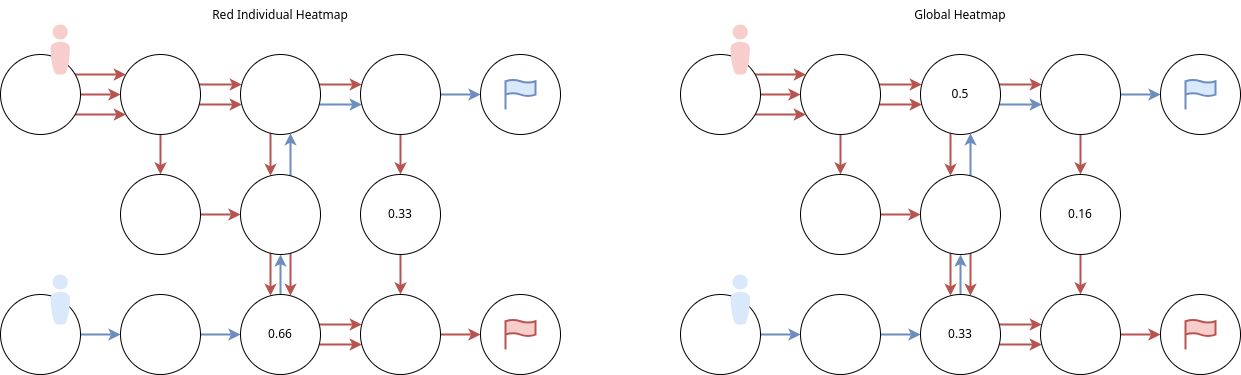
\includegraphics[width=11cm]{img/global_heatmap_p4.drawio.png}
    \end{figure}
\end{frame}


\begin{frame}{Global Heatmap example 5/5}
    \begin{figure}[H]
        \centering
        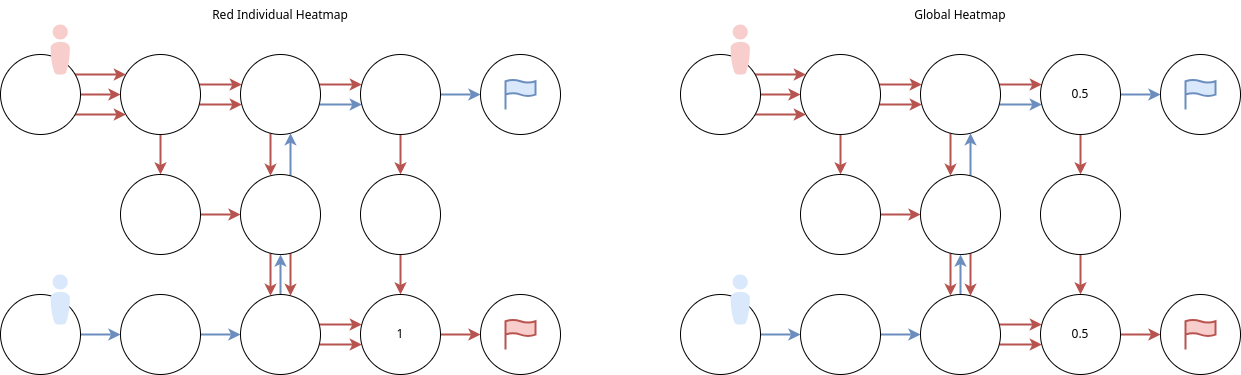
\includegraphics[width=11cm]{img/global_heatmap_p5.drawio.png}
    \end{figure}
\end{frame}



\begin{frame}{Path Elimination Approaches Summary}
    \textbf{Eliminate paths based on heatmaps:}

            \begin{itemize}
                \item \textbf{Unique Heatmap Values:}
                    \begin{itemize}
                        \item Order assignments by global heatmap values.
                        \item Identify critical vertices and eliminate paths containing them.
                    \end{itemize}
                \item \textbf{Threshold-based Elimination:}
                    \begin{itemize}
                        \item Define thresholds (\(\mathcal{H}\)) based on various properties.
                        \item A vertex is denoted critical if its global heatmap value is above the threshold
                    \end{itemize}
                \item \textbf{Sums of Global Heatmap Values:}
                    \begin{itemize}
                        \item For every path, we sum the value of each global heatmap value the paths goes on
                        \item We eliminate \(k\) paths based on the summed value 
                    \end{itemize}
            \end{itemize}
\end{frame}



\begin{frame}{An example}
    \begin{figure}[H]
        \centering
        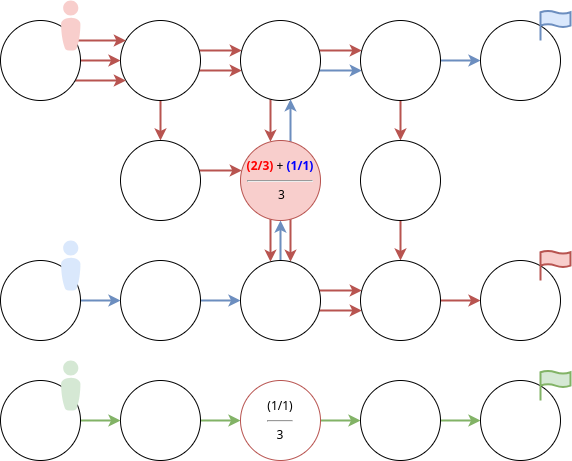
\includegraphics[width=\widthimg]{img/pe_one_heatmap_value_example.drawio.png}
    \end{figure}
\end{frame}





\subsection{Path Selection}
\begin{frame}{Path Selection: towards (partial) solving}
    In the end, what paths are we using? 


    \begin{itemize}
        \item Objective 1: Identify a conflict-free partial plan \(\hat{\Pi}\)
        \begin{itemize}
            \item At most one path per agent 
        \end{itemize}
        \item Objective 2: Create a subgraph 
        \begin{itemize}
            \item At least one path per agent
        \end{itemize}
    \end{itemize}
\end{frame}
